% !TEX root = tracking.tex
\section{Numerical examples} \label{sec:results}

In this section, we demonstrate the FaSTrack framework in three numerical examples involving a 5D car tracking a Dubins car model with the FSM planner, a 10D quadrotor tracking a single integrator model with the RRT planner, and an 8D quadrotor tracking a double integrator model with the MPC planner.
In each example, obstacles in the environment are \textit{a priori} unknown, and are revealed to the vehicle when they are sensed.
Whenever, obstacle map is updated, the planner re-plans a trajectory in real-time.
In this paper, the details of sensing are kept as simple as possible; we aim to only demonstrate our framework for real-time guaranteed safe planning and re-planning.
In general, any other planner can be used for planning in unknown environments, as long as planning and re-planning can be done in real-time.

For each example, we first describe the tracking and planning models. 
Next, we present the relative dynamics as well as the precomputation results. 
Afterwards, we briefly describe the planning algorithm and how obstacles are sensed by the vehicle. 
Finally, we show trajectory simulation results.

\subsection{5D-3D example with FSM planner \label{sec:reach_planner}}

For our first example, we demonstrate the combination of fast planning and provably robust tracking by combining fast sweeping method (FSM) \cite{Takei2013} with our computed TEB. 
FSM is an efficient optimal control-based planner for car-like systems, and provides numerically convergent globally optimal trajectory in real-time.

In this example, we use FSM to perform real-time planning for the 3D kinematic car model, whose trajectory is tracked by the 5D car model.
The dynamics of these models are given in \eqref{eq:5D_and_3D_dyn}.
The parameters are chosen to be $a \in [-0.5, 0.5]$, $|\alpha|\le 6$, $\hat v = 0.1$, $|\hat\omega|\le 1.5$, $|\dstb_x|, |\dstb_y|, |\dstb_\alpha|\le0.02$, $|\dstb_a| \le 0.2$.

\subsubsection{Offline computation}

Using the relative system dynamics given in \eqref{eq:5D_and_3D_rdyn}, we defined the error function to be $\errfunc(\rstate) = x_\rstate^2 + y_\rstate^2$, and computed $\valfunc_\infty(\rstate)$, which is shown in Fig. \ref{fig:vf_TEB:5D3D}.
The minimum of the value function was approximately $\underline\valfunc = $

The top left plot shows the TEB $\TEB_{\pstate, \infty}$, which is obtained from \eqref{eq:TEBp:inf}, in green.
The tracking model, which represents the system of interest, must apply the optimal control \eqref{eq:opt_ctrl} when it is on the green boundary.
The cross sectional area of the TEB is the largest area in when $\theta_r = 0, \pi$. 
This agrees with intuition, since at these $\theta_r$ values the 5D car model is either aligned with or opposite to the 3D car model.
Since the 5D car is able to move both forward and backward, these two alignments make tracking the easiest.
For the same reasoning, the cross sectional area is the smallest at $\theta_r = -\pi/2, \pi/2,$ etc.

The magenta and cyan planes indicate slices of the TEB at $\theta_r = \pi/2, -3\pi/4$, respectively.
With these $\theta_r$ values fixed, corresponding projections of the value function onto $(x_r, y_r)$ space are shown in the top right and bottom left plots.
Here, $\underline\valfunc$ is shown as the gray plane, with  the intersection of the gray plane and the value function projection shown by the curve in the value $=0$ plane. 
These curves are slices of $\TEB_{\pstate, \infty}$ at the $\theta_r = \pi/2, -3\pi/4$ levels.


\subsubsection{Online sensing and planning}
Besides planning a trajectory to the goal, the car must also sense obstacles in the vicinity. For illustration, we chose a simple virtual sensor that reveals obstacles within a range of $r$ meters.

Once an obstacle is sensed, the FSM planner replans the trajectory while taking into account all obstacles that have been sensed so far. 
To ensure that the 5D car does not collide with the obstacles despite error in tracking, planning is done with respect to augmented obstacles that are ``expanded'' from the sensed obstacles by $\underline\valfunc$ in $(x,y)$ position space.

\MCnote{Online computation details (time etc.)}

\subsubsection{Simulations}

The Dubins car parameters are

The control bounds for the 5D car are $a \in []$, $|\alpha| < $.

The disturbance bound is $\|(d_x, d_y)\|_2 < $.

The sensing range is $r = $ meters.

We used a C implementation of FSM.

Computation times:
\begin{itemize}
\item === TOTAL ===
\item  512 iterations in 637.5527 seconds
\item 1.2452 seconds per iteration on average
\item === PLANNING ===
\item 512 iterations in 33.5683 seconds
\item 0.0656 seconds per iteration on average
\item === TRACKING ===
\item 512 iterations in 0.8991 seconds
\item 0.0018 seconds per iteration on average
\end{itemize}

On an unoptimized MATLAB implementation on a desktop computer with a Core i7-2600K CPU, each iteration took approximately ?? ms on average. Most of this time is spent on planning: obtaining the tracking controller took approximately ?? ms per iteration on average. The frequency of control was once every ?? ms.

\MCnote{Fig. ?? shows the simulation results. 
Four time snapshots are shown. The initial position is $(-12, 0, 0)$, and the goal position is $(12, 0, 0)$. The top left subplot shows the entire trajectory from beginning to end. In all plots, a magenta star represents the position of the planning model; its movement is based on the paths planned by RRT, and is modeled by a 3D holonomic vehicle with a maximum speed. The blue box around the magenta star represents the tracking error bound.}

\begin{figure}
  \label{fig:5D3Dsim}
  \centering
  \begin{subfigure}[t]{0.49\columnwidth} \label{fig:5D3Dsim:1}
    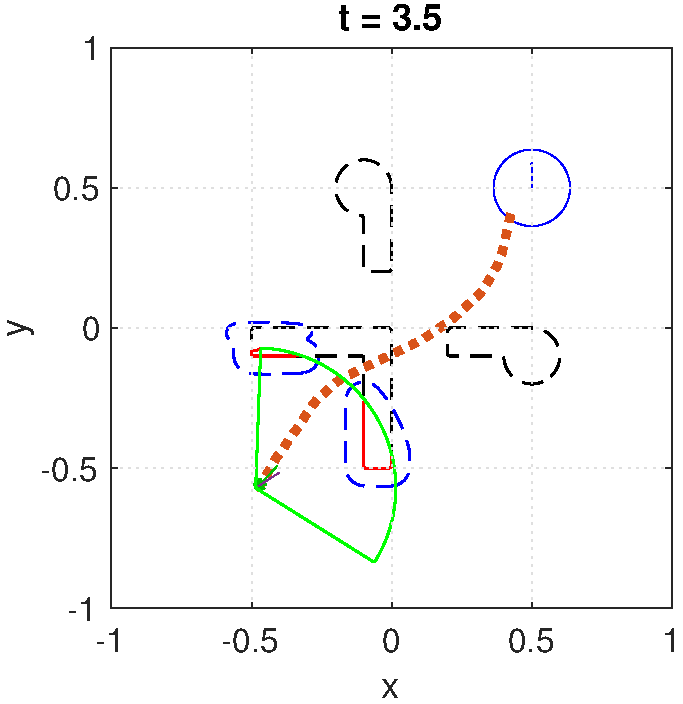
\includegraphics[width=\columnwidth]{fig/P5D_Dubins/36}
  \end{subfigure}
  \begin{subfigure}[t]{0.49\columnwidth} \label{fig:5D3Dsim:2}
    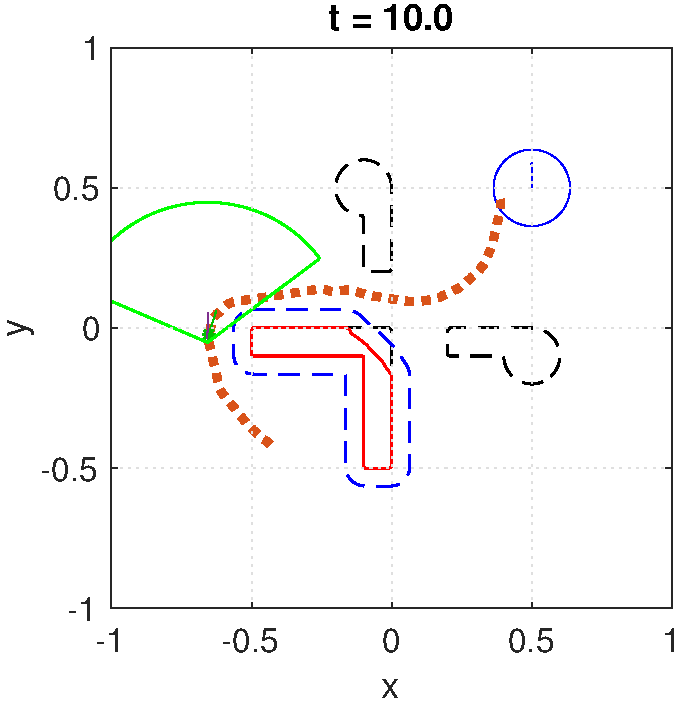
\includegraphics[width=\columnwidth]{fig/P5D_Dubins/101}
    \caption{}
  \end{subfigure}  

  \begin{subfigure}[t]{0.49\columnwidth}\label{fig:5D3Dsim:3}
    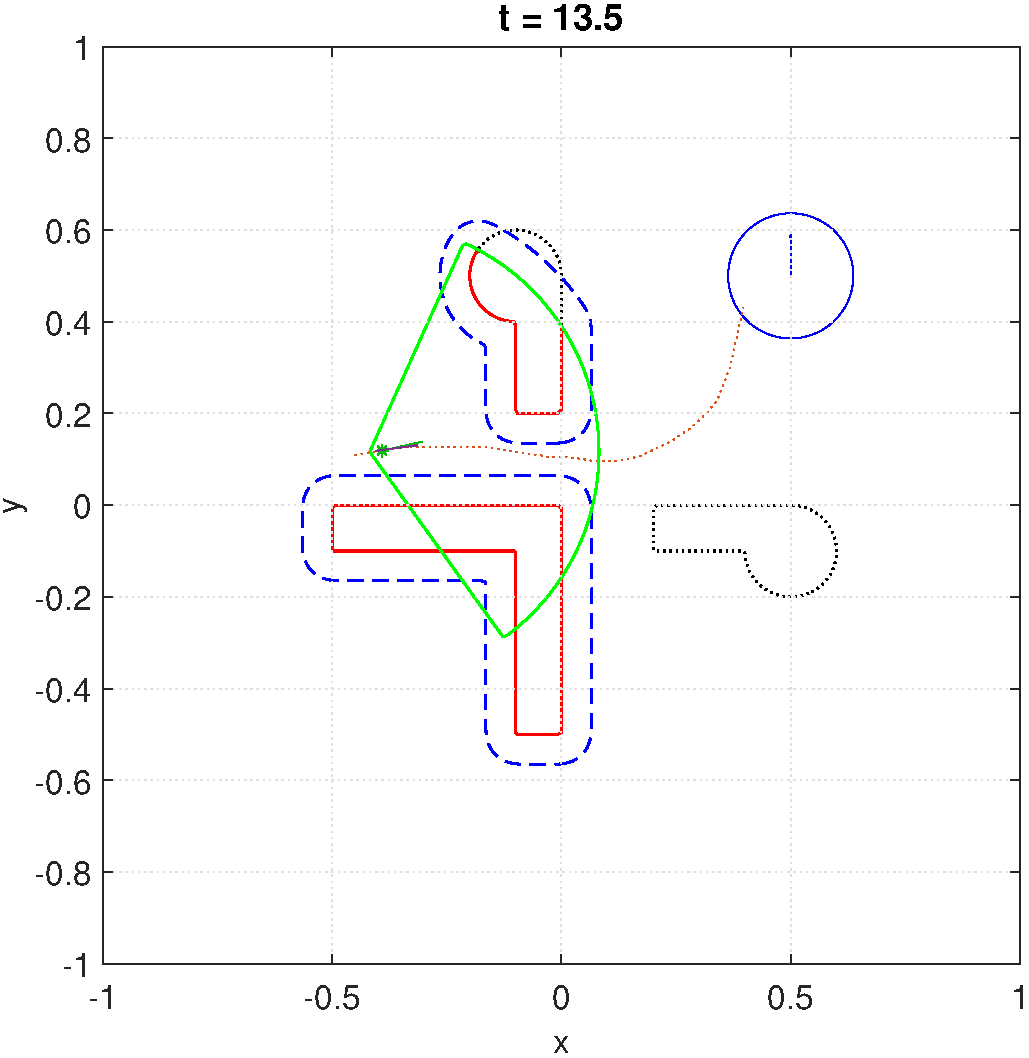
\includegraphics[width=\columnwidth]{fig/P5D_Dubins/136}
    \caption{}
  \end{subfigure}
  \begin{subfigure}[t]{0.49\columnwidth}\label{fig:5D3Dsim:4}
    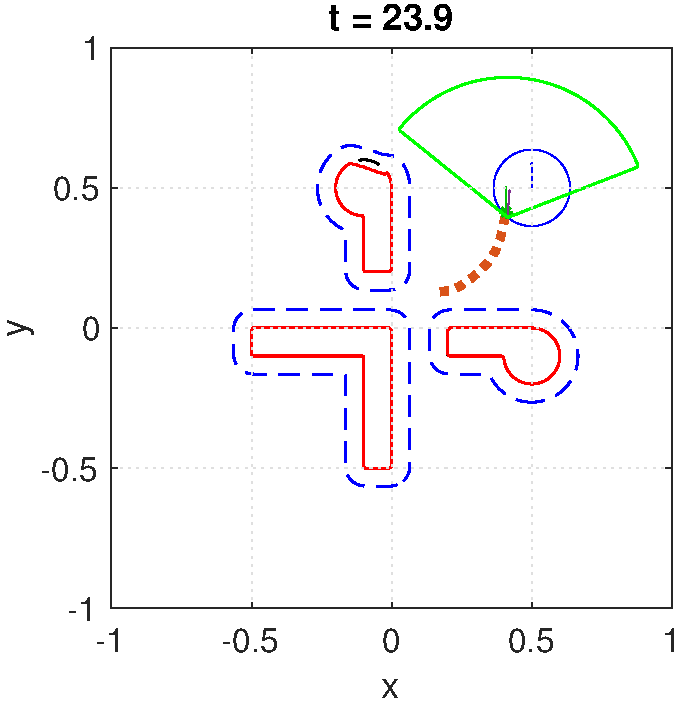
\includegraphics[width=\columnwidth]{fig/P5D_Dubins/240}
    \caption{}
  \end{subfigure}
  \caption{}
\end{figure}